% !TEX encoding = UTF-8 Unicode
\kap{The Editor}
\ukap{The Main View}
%Die ''Bühne'' macht den größten Teil des Editors aus. Auf ihr können Plugins, Module sowie Regler platziert und bedient werden.
The main view is the largest part of the VSTForx editor, use it to place and control plugins, modules and knobs.
\ukap{Moving And Connecting}
\uukap{\label{corona}The Corona Field}
The problem, which appears especially when using knobs, is that we can do three actions: moving, using and connecting. But we have only one mouse button! 
\emph{(The right mouse button is for translating the view. Modificator keys such as “shift” or “ctrl” are problematic because there is lack of keyboard support in some host applications.)}
\\\\
The solution to this problem is the “corona” field which appears when you hover over an object. There are “two” corona types:
\\
\begin{figure}[]
\begin{center}
	
\includegraphics[]{../graphics/node-corona}
\caption{the node corona}
\label{nodec}
\end{center}
\end{figure}
\begin{figure}[]
\begin{center}
	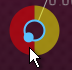
\includegraphics[]{../graphics/knob-corona}
\caption{the knob corona}
\label{knobec}
\end{center}
\end{figure}

\begin{description}
	\item[The Node Corona]  (figure \ref{nodec}) The node corona which is a single (yellow) field around a node. With draggin this yellow zone you are able to move the node around. Connecting will be approached by dragging the mouse over the node.
	\item[The Knob Corona] (figure \ref{knobec}) The knob corona is a double sided field (red/yellow) around a knob. The yellow side is still for moving the knob. The red side is for connecting the knob with another knob. To manipulate (use) the knob just use the knob as expected.\end{description}

\ukap{Main Entry/Exit}
%Ähnlich real existierender Hardware, bietet VSTForx frei verdrahtbare Schnittstellen für externe und interne Module: die Ein- und Ausgänge. Ein Eingang lässt sich mit einem beliebigen Ausgang verbinden und ein Ausgang mit einem beliebigen Eingang. 
\paragraph{Main Entry} (
\includegraphics[scale=0.5, bb = 0 15 40 0]{../graphics/InputNode}) \\\\
%Hier liegt das Audio-Signal, an welches von einer Hostanwendung an VSTForx gesendet wird.
From here comes the audio signal of your host application.
\paragraph{Main Exit} (
\includegraphics[scale=0.5,bb = 0 15 40 0]{../graphics/OutputNode}) \\\\
Here will the audio signal sent back to the host application.
